\chapter{المهام}
\label{ch:tasks}

\section{ماذا ستنجز؟}

يساعدك تطبيق المهام على تحويل العمل المطلوب إلى مهمة واضحة لها مسؤول وموعد ونتيجة متوقعة. يتابع الموظف ما أُسند إليه، ويراجع المدير التقدم والعوائق، بينما يهيّئ المسؤول أنواع المهام ومسارات حالاتها.

\begin{rcnote}[مثال: شركة الأفق]
تتابع سارة الخطيب تجهيز زيارة فرع حلب في شركة الأفق، ويساعدها عمر حداد بإعداد قائمة الزيارة. هذا المثال افتراضي، أما صور الفصل فتعرض سجلات اختبار مستقلة عنه.
\end{rcnote}
\begin{figure}[H]
\centering
\begin{tikzpicture}[node distance=0.5cm]
\node[stepBox] (a) {\RL{المجموعة: مكان العمل}};
\node[stepBox,below=of a] (b) {\RL{المهمة: نتيجة ومسؤولية}};
\node[stepBox,below=of b] (c) {\RL{التحديث: نتيجة وحالة}};
\draw[flowsTo] (a) -- (b);
\draw[flowsTo] (b) -- (c);
\end{tikzpicture}
\rclegend
\caption{تسلسل العمل اليومي في المهام}
\label{fig:tasks-overview-flow}
\shotnote{يبيّن الشكل التسلسل المعتاد للعمل: تبدأ من المجموعة التي تضم عملك، ثم تفتح المهمة لتعرف النتيجة المطلوبة ومسؤولها، ثم تحدّث حالتها وتسجّل ما أنجزت. هذه خطوات يؤديها المستخدم بنفسه، فالمجموعة لا تغيّر حالة المهمة تلقائياً.}
\end{figure}

\begin{figure}[H]
\centering
\begin{tikzpicture}[node distance=0.5cm]
\node[entity] (task) {\RL{المهمة}};
\node[entityOpt,below right=0.7cm and 0.3cm of task] (record) {\RL{سجل مرتبط}};
\node[entityOpt,below left=0.7cm and 0.3cm of task] (other) {\RL{مهمة أخرى}};
\draw[dependsOnOpt] (task.south) -- ++(0,-0.3) -| (record.north);
\draw[dependsOnOpt] (task.south) -- ++(0,-0.3) -| (other.north);
\end{tikzpicture}
\rclegend
\caption{روابط تضيف سياقاً للعمل}
\label{fig:tasks-models}
\shotnote{يوضّح الشكل أن المهمة قد ترتبط بسجل آخر في كيان أو بمهمة أخرى، فيعرف الفريق مصدر العمل وما يتصل به. هذه الروابط اختيارية في الأصل، لكن نوع المهمة قد يشترط بعضها عند الإنشاء أو الإكمال. أما علاقة الحجب فقد تمنع إكمال المهمة، بخلاف الرابط العادي.}
\end{figure}

\section{دليل صفحات المهام}
\label{sec:tasks-pages}

\begin{figure}[H]
\centering
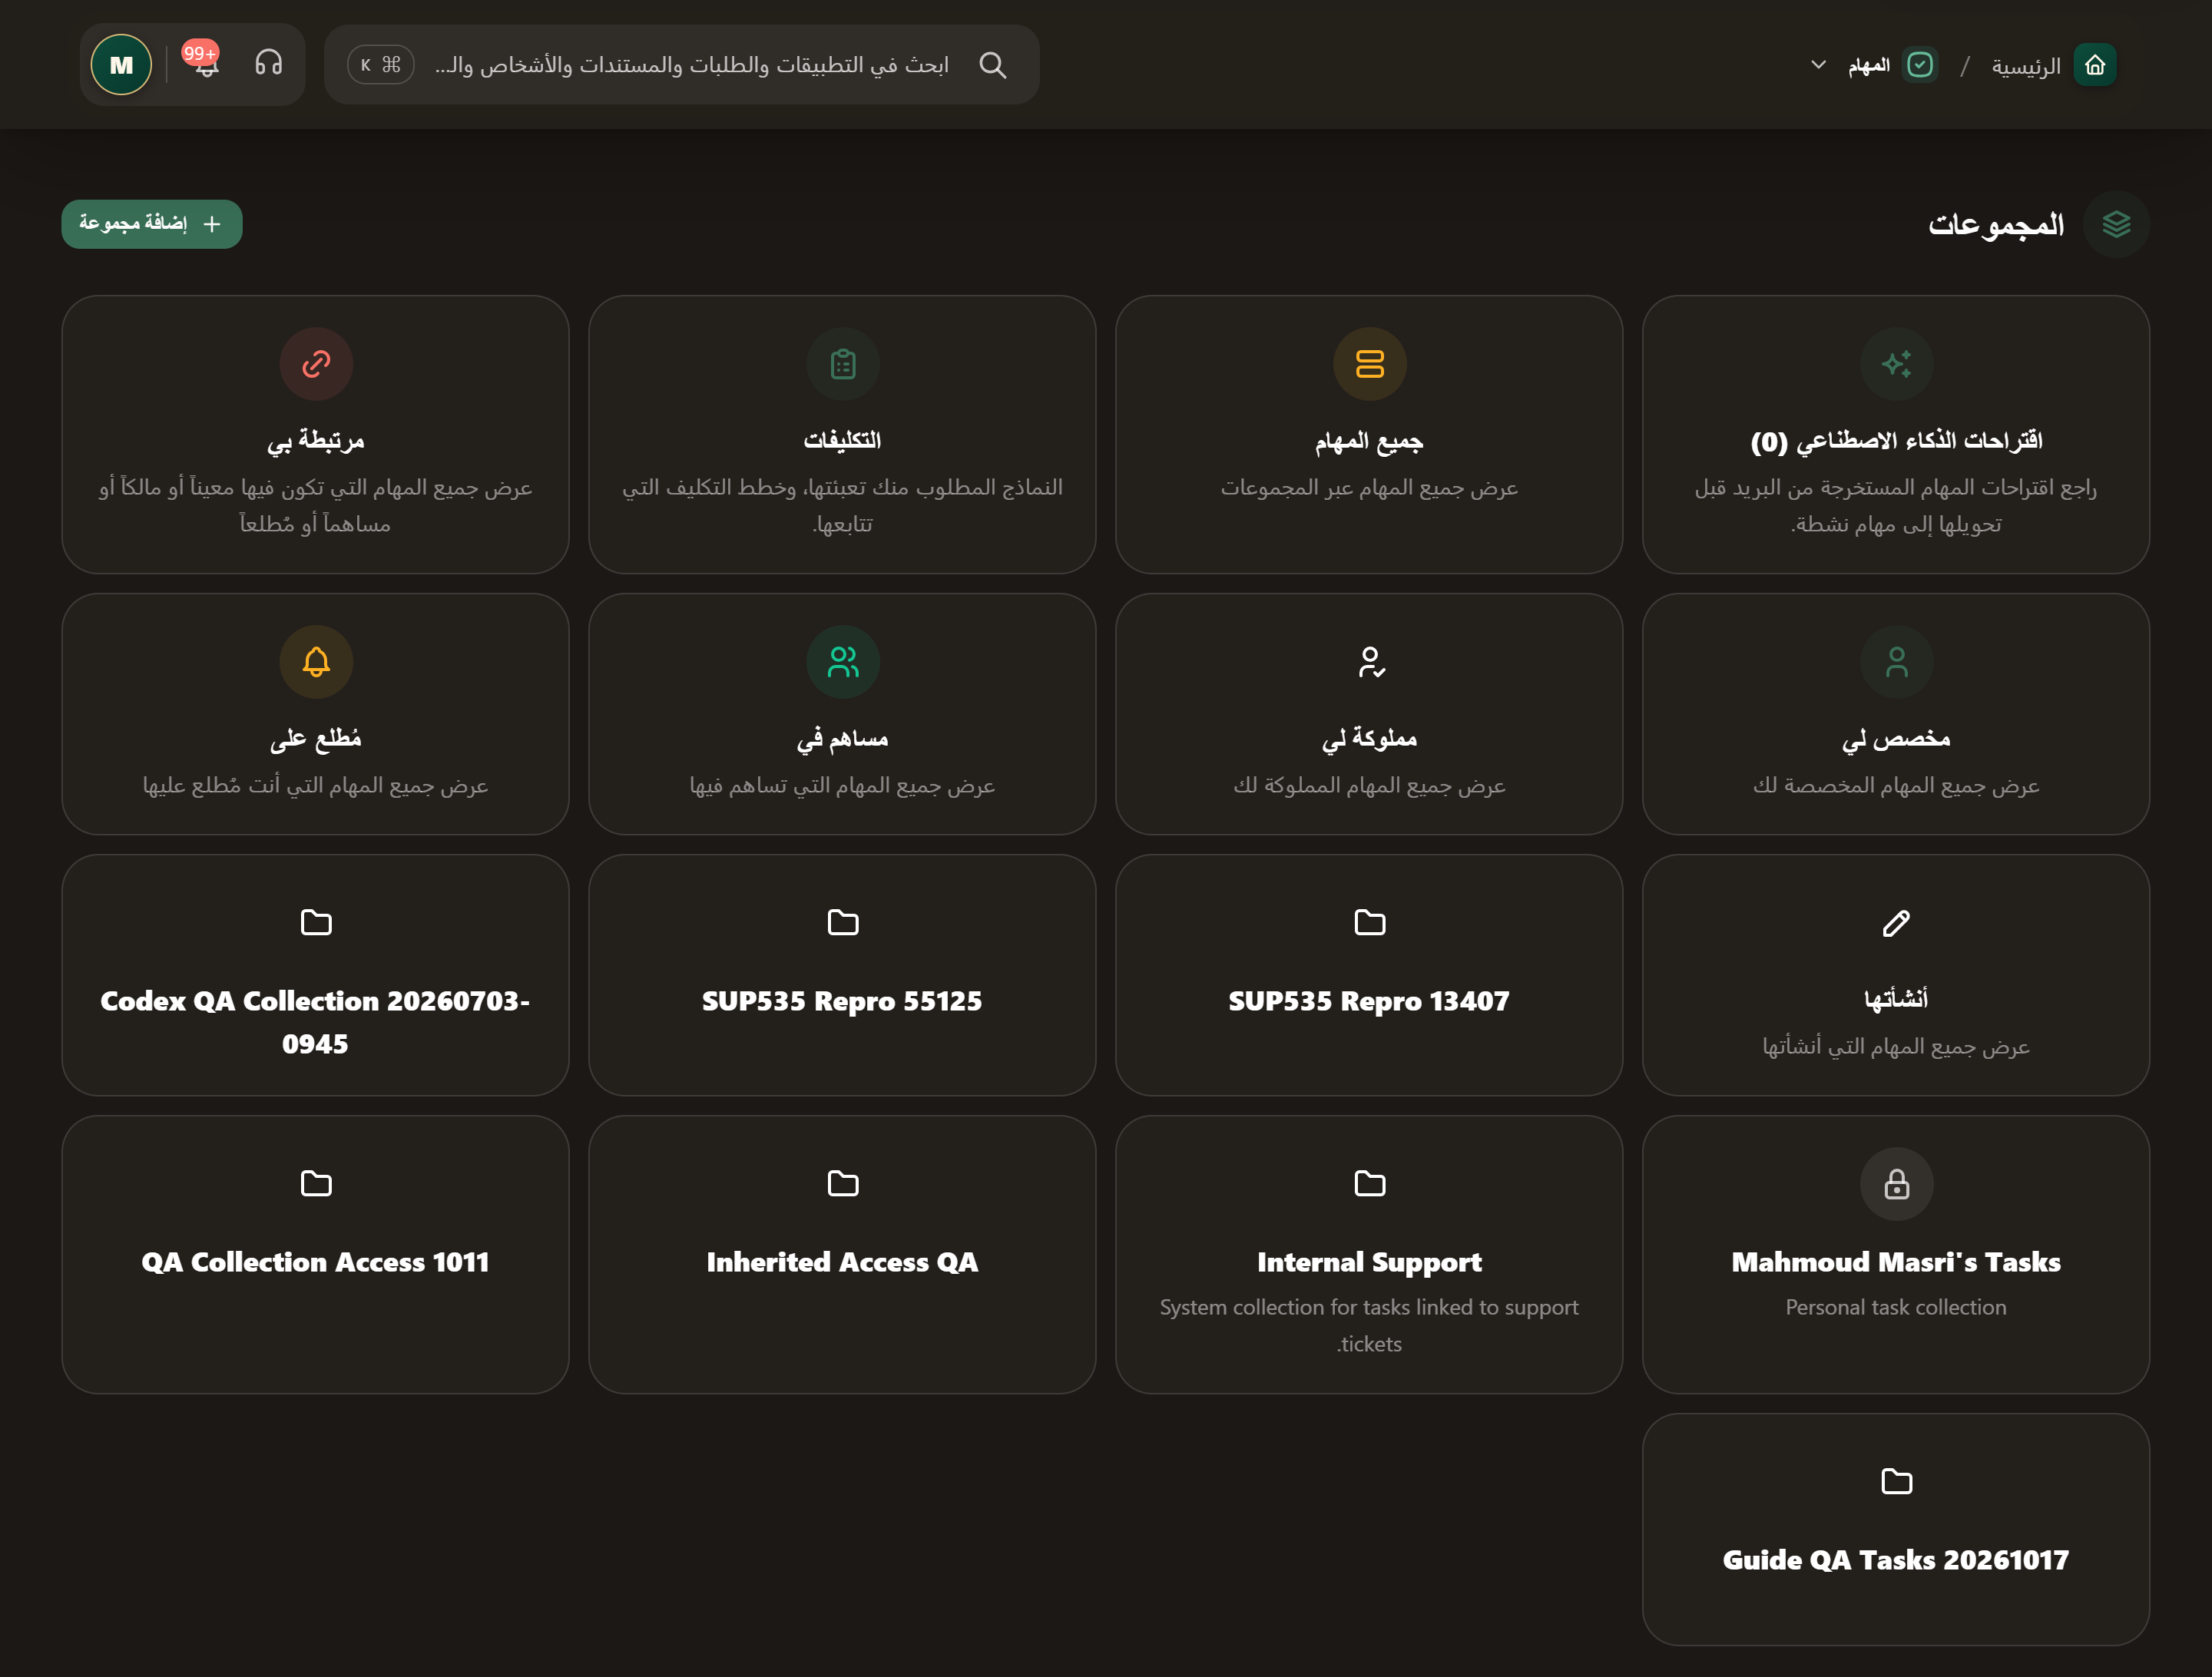
\includegraphics[width=0.95\linewidth,height=0.72\textheight,keepaspectratio]{figures/screens/ch04-collections-ar.png}
\caption{صفحة «المجموعات»: مدخل تطبيق المهام}
\label{fig:tasks-directory-screen}
\shotnote{تعرض صفحة «المجموعات» بطاقات جاهزة مثل «جميع المهام» و«مخصص لي» إلى جانب المجموعات التي أنشأتها المؤسسة، فتبدأ من البطاقة التي تخص عملك. أما «التكليفات» و«اقتراحات الذكاء الاصطناعي» فلكل منهما بطاقة مستقلة، ويشرح الدليل كلاً منهما في صفحة خاصة.}
\end{figure}

ابدأ بالمجموعات والعروض، ثم انتقل إلى إنشاء المهمة ومتابعتها وربطها بغيرها، واستخدم المهام الكبرى عندما تقسّم عملاً واسعاً. أما الاقتراحات والتكليفات فمساران متخصصان، والإعدادات من شأن المسؤول. وتشرح بعض الصفحات التالية تبويبات أو أدوات داخل المهمة، لا صفحات مستقلة في التطبيق.

\begin{table}[H]
\centering
\caption{من العمل اليومي إلى التهيئة}
\label{tab:tasks-pages-all}
\begin{tabularx}{\linewidth}{R{4.2cm} Y}
\rcHeaderRow
\thh{الصفحة} & \thh{ماذا تقدم هذه الصفحة؟}\\
المجموعات & تجمع المجموعة مهام العمل الواحد في مكان واحد.\\
عروض المهام & يغيّر العرض طريقة العثور على المهام ومتابعتها.\\
إنشاء المهمة وتفاصيلها & تسجّل المهمة النتيجة المطلوبة ومن يتولاها.\\
التقدم والنتائج والتواصل & تجمع المهمة ما أُنجز وما يعيق العمل وما يطلبه الزملاء بعضهم من بعض.\\
العلاقات والسجلات المرتبطة & تربط العلاقات المهمة بمصدر العمل أو بما يثبت إنجازه أو بمهمة أخرى.\\
المهام الكبرى & تجمع المهمة الكبرى عدة مهام تخدم نتيجة أوسع.\\
اقتراحات الذكاء الاصطناعي & الاقتراح عمل مستخرج من سياق البريد، ويحتاج إلى مراجعة قبل أن يصبح مهمة فعلية.\\
التكليفات & تعرض التكليفات النماذج المطلوب منك تعبئتها والعمل المرتبط بها.\\
إعدادات المهام & تحدّد إعدادات المهام أنواع العمل وتصنيفاته والعلاقات المتاحة.\\
قوالب الحالات & يحدّد قالب الحالة مراحل العمل والانتقالات بينها.\\
\end{tabularx}
\end{table}
